\documentclass[article]{jss}
\usepackage{amsmath,bm,amssymb,dsfont}
%\usepackage{pdfdraftcopy}
%\usepackage{/Library/Frameworks/R.framework/Resources/share/texmf/Sweave}

\DeclareMathOperator*{\argmin}{arg\,min}
\DeclareMathOperator*{\se}{se}

% To change the R input/output style:

\definecolor{Soutput}{rgb}{0,0,0.56}
\definecolor{Sinput}{rgb}{0.56,0,0}
\DefineVerbatimEnvironment{Sinput}{Verbatim}
{formatcom={\color{Sinput}},fontsize=\footnotesize, baselinestretch=0.75}
\DefineVerbatimEnvironment{Soutput}{Verbatim}
{formatcom={\color{Soutput}},fontsize=\footnotesize, baselinestretch=0.75}

 
%%%%%%%%%%%%%%%%%%%%%%%%%%%%%%
%% declarations for jss.cls %%%%%%%%%%%%%%%%%%%%%%%%%%%%%%%%%%%%%%%%%%
%%%%%%%%%%%%%%%%%%%%%%%%%%%%%%

%% almost as usual
\author{Robert Ferstl\\University of Regensburg \And 
        Josef Hayden\\ University of Regensburg}
\title{Zero-Coupon Yield Curve Estimation\\ with the Package \pkg{termstrc}}

%% for pretty printing and a nice hypersummary also set:
\Plainauthor{Robert Ferstl, Josef Hayden} %% comma-separated
\Plaintitle{Zero-Coupon Yield Curve Estimation with the Package termstrc} %% without formatting
\Shorttitle{Zero-Coupon Yield Curve Estimation with the Package termstrc} %% a short title (if necessary)

%% an abstract and keywords
\Abstract{
Zero-coupon yield curves and credit spread curves are important inputs for various financial models, e.g. pricing of securities, risk management, monetary policy issues. Since zero-coupon rates are rarely directly observable, they have to be estimated from market data, e.g. of existing coupon bonds. The literature broadly distinguishes between parametric and spline-based estimation methods for the zero-coupon yield curve. Our package consists of several widely-used approaches, i.e. the parametric \cite{Nelson1987} method with the \cite{Svensson1994} extension, and the \cite{McCulloch1975} cubic splines approach. Moreover, we implement the traditional way of credit spread calculation, where individually estimated zero-coupon yield curves are substracted from a risk-free reference curve. Goodness-of-fit tests are provided to compare the results of the different estimation methods. We illustrate the usage of our functions by practical examples with data from European and CEE government bonds, and European corporate bonds.
}
\Keywords{fixed income, term structure estimation, credit spreads, \proglang{R}}
\Plainkeywords{fixed income, term structure estimation, credit spreads, R} %% without formatting
%% at least one keyword must be supplied

%% publication information
%% NOTE: Typically, this can be left commented and will be filled out by the technical editor
%% \Volume{13}
%% \Issue{9}
%% \Month{September}
%% \Year{2004}
%% \Submitdate{2004-09-29}
%% \Acceptdate{2004-09-29}

%% The address of (at least) one author should be given
%% in the following format:
\Address{
  Robert Ferstl\\
  Department of Finance\\
  University of Regensburg\\
  93053 Regensburg, Germany\\
  E-mail: \email{robert.ferstl@wiwi.uni-regensburg.de}\\
  URL: \url{http://www-finanzierung.uni-regensburg.de}\\
  
  Josef Hayden\\
  Department of Finance\\
  University of Regensburg\\
  93053 Regensburg, Germany\\
  E-mail: \email{josef.hayden@wiwi.uni-regensburg.de}\\
  URL: \url{http://www-finanzierung.uni-regensburg.de}
}
%% It is also possible to add a telephone and fax number
%% before the e-mail in the following format:
%% Telephone: +43/1/31336-5053
%% Fax: +43/1/31336-734

%% for those who use Sweave please include the following line (with % symbols):
%% need no \usepackage{Sweave.sty}

%% end of declarations %%%%%%%%%%%%%%%%%%%%%%%%%%%%%%%%%%%%%%%%%%%%%%%


\begin{document}

%% include your article here, just as usual
%% Note that you should use the \pkg{}, \proglang{} and \code{} commands.
%% Note: If there is markup in \(sub)section, then it has to be escape as above.

\section{Introduction}

\textcolor{red}{
\begin{itemize}
\item central banks are not so concerned with accuracy with regard to pricing securities
\end{itemize}
}

% Defintion of the problem

The term structure of interest rates or the zero-coupon yield curve is the relationship between fixed income investments with only one payment at maturity, and the time to maturity of these cashflows. It is used in different areas of application, e.g. risk management, financial engineering, monetary policy issues. The zero-coupon yield curve is the basis to value other fixed income instruments. Basically, we can calculate the net present value (NPV) of any cash flow with it. For example, the fair price of a bond is just the sum of its discounted future coupon and redemption payments. By comparing it to the price on the market, we can identify mispriced securities. The numerous areas of application for the term structure of interest rates has lead to a fairly large amount of publications by researchers and practitioners.

Before we come to the problem of zero-coupon yield curve estimation, let us introduce the definitions of a few basic terms used in the fixed income literature. A \emph{discount bond} or \emph{zero-coupon bond} is a fixed income investment with only one payment at maturity. The \emph{spot rate} or \emph{zero-coupon rate} is the interest paid on a discount bond. With continuous compounding the fair price of a discount bond paying \$1 at maturitydate  $m_t$ is given by

\begin{equation}
  \label{eq:pricediscountbond}
  p(m_t)=e^{s(m_t)m_t}
\end{equation}

Therefore, the \emph{spot curve} (or \emph{zero-coupon yield curve}) shows the spot rates for different maturities. The spot rate is the interest paid for investments that start today ($t=0)$. The \emph{forward rate} $f(t',T)$ is the interest contracted now to be paid for an future investment between the time $t'$ and $T$. The forward rate as a function of maturity is the \emph{forward curve}. With continuous compounding, we have the following relationship between spot rates and forward rates.

\begin{equation}
  \label{eq:relspotforward}
  e^{s(m_{t'}) m_{t'}}e^{f(t',T)(m_T-m_{t'})} = e^{s(m_T) m_T}
\end{equation}
We can solve (\ref{eq:relspotforward}) for the forward rate.

\begin{equation}
  \label{eq:forwardrate}
  f(t',T) = \frac{s(m_T)m_T - s(m_{t'})m_{t'}}{m_T-m_{t'}}
\end{equation}

The \emph{instantaneous forward rate} describes the return for an infinitesmal investment period after the date $t'$.

\begin{equation}
  \label{eq:instforw}
  f(t') = \lim_{T\rightarrow t'}f(t',T)
\end{equation}

Another interpretation is as the marginal increase in the total return from a marginal increase in the length of the investment period. Therefore, the spot rate can be seen as average of the instantaneous forward rates.

\begin{equation}
  \label{eq:avgforwardrate}
  s(m_t)=\frac{1}{m_t}\int_0^{m_t}f(s)ds
\end{equation}

In practice, we can only obtain zero-coupon rates for a limited amount of maturities directly from the market. Therefore, we have to estimate them from observed prices of \emph{coupon bonds}. The following information is typically available on the market: the clean price $p_c$, the cashflows $c_t$ (coupons and redemption payment) and their maturity dates $m_t$. An investor who wants to buy the bond has to pay the dirty price $p_d$ which consists of the quoted market price (clean price) $p_c$ and the accrued interest $a$. This is the amount of interest that has accumulated since the last coupon payment. Similar to \eqref{eq:pricediscountbond}, the bond pricing equation under continuous compounding is the present value of all cash flows.

\begin{equation}
  \label{bondpriceeq}
  p_c+a = \sum_{t=1}^T \ c_t e^{-s(m_t)m_t}
\end{equation}

An equivalent formulation makes use of the \emph{discount factors} $d_t=\delta(m_t)=e^{-s(m_t)m_t}$. The continuous \emph{discount curve} $\delta(\cdot)$ is formed by interpolation of the discount factors.


\begin{equation}
  \label{bondprceq2}
  p_c+a=\sum_{t=1}^T \ c_t \delta(m_t) 
\end{equation}
Each payment (coupons and redemption) has the structure of a discount bond. This makes it possible to relate the coupon bond prices to the spot and the forward curve. The usual way to compare coupon bonds with different maturities is to calculate the internal rate of return of the cash flows. The so-called \emph{yield-to-maturity} (YTM) is the solution for $y$ in the following equation.

\begin{equation}
   \label{yield}
   p_c+a=\sum_{t=1}^T \ c_t e^{-ym_t}
 \end{equation}

As can be seen from \eqref{eq:pricediscountbond}, the YTM for a discount bond is equal to the spot rate. This is not true for coupon bonds. Plotting just the yield-to-maturity for coupon bonds with different maturities does not result in a yield curve which can be used to discount cash flows or price any other fixed income security except the bond from which it was calculated. Therefore, estimating the term structure of interest rates from a set of coupon bonds can not be seen as a simple curve fitting of the YTMs.

We have seen before that the spot curve, the forward curve and the discount curve are implied by each other. The following estimation procedures try to approximate one of them, from which it is possible to calculate the other ones. The simplest method to obtain spot rates from a sample of coupon bonds is bootstrapping. This is an iterative technique based on the pricing equation for a coupon bond. It works only when all cashflows have the same maturity intervals \citep[see, e.g.][]{Hagan2006}. Therefore, other estimation procedures are needed. Usually, the following features are required from an estimated yield curve. It should price the underlying bonds correctly and result in a continuous spot and forward curve. 

\cite{BIS2005} contains a survey about zero-coupon yield curve estimation procedures among central banks. It turns out that the following two approaches are widely used. The first are parametric cubic splines for the discount function proposed by \cite{McCulloch1971, McCulloch1975}. The second method is based on a parsimonious specification of the forward curve with a family of exponential polynomials developed by \cite{Nelson1987} and extended by \cite{Svensson1994}. Both approaches minimize the price/yield errors, however, estimation procedures are different, e.g. they can involve weightings of the errors, the objective function can become nonlinear.

There are several extensions available for the two methods mentioned above. \cite{Vasicek1982} fit the discount function with exponential splines. \cite{Fisher1995} proposed a smoothing spline for which \cite{Waggoner1997} introduced a roughness penalty varying across maturities. Different weightings for the objective function of the exponential polynomial families can be found in \cite{Soederlind1997}. Several works compare the performance of different term structure estimation methods, \citep[see e.g.][]{Bliss1997, Bolder1999, Ioannides2003}.

In practice, new data for the yield curve is available everyday, and it is obvious to recalibrate the estimation in a dynamic way or even try to forecast the future parameters. \cite{Diebold2006} propose an approach that is based on the Nelson-Siegel model. Term structure estimation procedures do not have to be consistent with intertemporal interest modeling by diffusion processes \citep[see, e.g.][]{Bjoerk1999, Filipovic1999}. For a consistent and arbitrage-free version of the Nielsen-Siegel model, which can be used for pricing fixed income derivatives, see \cite{Krippner2006}.   

In this paper, we give a short overview about the topic of term structure estimation methods and introduce the package \pkg{termstrc} which is written in the \proglang{R} system for statistical computing \citep{R2008}. It is available from the Comprehensive \proglang{R} Archive Network at \url{http://CRAN.R-project.org/}. The package contains an implementation of the two most widely-used methods for zero-coupon yield curve estimation from market data of coupon bonds, i.e. the parametric \cite{Nelson1987} method with the \cite{Svensson1994} extension, and the \cite{McCulloch1975} cubic splines approach. The software provides detailed summaries about the estimation results as well as graphical outputs of spot, forward and credit spread curves.



%%% Local Variables: 
%%% mode: latex
%%% TeX-master: "jss-termstrc"
%%% End: 

\section{Zero-coupon yield curve estimation}

\subsection{Notation}
\label{sec:notation}

Let us establish the necessary notation for a market data set of coupon bonds. We denote an element-wise multiplication with ``$\cdot$'' and $( )'$ is the transpose of a matrix. $\bm{\iota}$ defines a column vector filled with ones.

\subsubsection*{Maturity matrix}

\begin{equation*}\label{maturitym}
\bm{M}_{\left[n\times m\right]}= \{m_{ij}\}
\end{equation*}

The number of rows $n$ is determined through the number of cashflows of the bond $j$ with the longest maturity. For each bond $j$ exists a column with the corresponding cashflow dates. Dates after the maturity of the bond $j$ are filled up with zeros till the maturity date of the bond with the longest maturity. One element $m_{ij}$ of the matrix  refers, therefore, to the maturity date of  the $i$-th cashflow of the $j$-th bond. 

\subsubsection*{Maturity vector}

We denote with $m_j$ the maturity of the last cashflow, i.e. the maturity of the $j$-th bond.

\begin{equation*}\label{weights}
    \bm{m}_{\left[1\times m\right]}= \{m_j\}
\end{equation*}

\subsubsection*{Cashflow matrix}


 \begin{equation*}\label{cashflowm}
\bm{C}_{\left[n\times m\right]}= \{c_{ij}\}
\end{equation*}

 The cashflow matrix is defined analogously to the maturity matrix.  One element $c_{ij}$  of the matrix refers to the $i$-th cashflow of the $j$-th bond. Note, that the last cashflow of a each bond includes the redemption payment.

\subsubsection*{Discount factor matrix}

 \begin{equation*}\label{discountm}
\bm{D}_{\left[n\times m\right]}= \{d_{ij}\}
\end{equation*}

The discount factor matrix is also defined analogously to the maturity matrix. One element $d_{ij}$ of the matrix refers to the discount factor associated with  the $i$-th cashflow of the $j$-th bond. The discount function $\delta(m_{i,j})$ returns the discount factor for a given maturity. We will see in the following sections several methods how to estimate it. From an economic point of view only positve interest rates make sense. This implies that the discount factors are nonnegative where the entries in the maturity matrix are greater zero. Remember, zero entries in the maturity matrix mean that for these points in time now cash flows are associated.

\subsubsection*{Clean price vector}

 \begin{equation*}\label{pc}
\bm{p}^c_{\left[1\times m\right]}= \{p^c_j\}
\end{equation*}

$p_{j}^c$ is the quoted market price of the $j$-th bond. It is given as percentage of the nominal value.

\subsubsection*{Accrued interest vector}

When an investor buys a bond, he will receive all its future cash flows. If the purchase occurs between two coupon dates, the seller must be compensated for the fraction of the next coupon, the so-called \emph{accrued interest}.

  \begin{equation*}\label{a}
\bm{a}_{\left[1\times m\right]}= \{a_j\}
\end{equation*}


In practice, the calculation depends on the used day-count convention, e.g. 30/360, Actual/360. A basic form for the $j$-th bond is as follows.

\begin{equation*}
    a_j= \frac{\mbox{number of days since last coupon payment}}{\mbox{number of days in current coupon period}}\cdot \mbox{coupon}_j
\end{equation*}
 	

\subsubsection*{Dirty price vector}

The dirty price vector is the sum of the clean price vector and the accrued interest vector.

\begin{displaymath}
\bm{p}=\bm{p}^c+\bm{a}
\end{displaymath}

The elements are denoted by 
\begin{equation*}\label{pd}
    \bm{p}_{\left[1\times m\right]}= \{p_j\}\,.
\end{equation*}


\subsubsection*{Yield-to-maturity vector}

This vector contains the yield-to-maturity described in \eqref{eq:yield}.

\begin{equation*}\label{pd}
    \bm{y}_{\left[1\times m\right]}= \{y_j\}\,.
\end{equation*}



\subsubsection*{Duration vector}

The time to maturity of a coupon bond should not be used as an indicator for the sensitivity of a bond's price against changes in the interest rate. One needs to account for the fact that coupons are paid during the life time of a bond. Therefore, we calculate the average maturity weighted by the present values of its cash flows. This concept is called (Macaulay) \emph{duration}.

\begin{equation*}
  \label{eq:macaulayduration}
  \bm{d}_{\left[1\times m\right]} = \frac{\bm{\iota}'(\bm{C}\cdot\bm{M}\cdot\bm{D})}{\bm{\iota}'(\bm{C}\cdot\bm{D})}
\end{equation*}

Here, the discount matrix $\bm{D}$ contains the disount factors calulated with the yield-to-maturity of each bond as in \eqref{eq:yield}.

\subsubsection*{Weights matrix}

In section \ref{sec:nels-svenss-meth}, we will use a weighting matrix for the estimation errors. It is constructed  as follows.

\begin{equation*}\label{weights}
    \bm{\Omega}_{\left[m\times m\right]}= \begin{pmatrix}
 \omega_1 & 0 &\cdots  &0  \\
 0 & \omega_2 &  & \vdots \\
 \vdots &  & \ddots & 0 \\
 0 &\cdots  &0  & \omega_m
\end{pmatrix}
\end{equation*}


Whereas $\omega_j$ is the weight for bond $j$ with duration $d_j$:

\begin{equation}
\label{eq:durationweight}
    \omega_j=\frac{\frac{1}{d_j}}{\sum_{i=1}^m\frac{1}{d_i}}
\end{equation}



\subsection{Estimation procedure}
\label{sec:estimation}

The simplest smoothing technique is linear interpolation. In many cases it is not appropriate for zero-coupon yield curve estimation, because it can lead to spikes in the forward rate curve, which is a problem from an economic point of view. Therefore, we use indirect estimation procedures that postulate a specific form for the spot rate function $s(m_t, \bm{b})$ or the discount function $\delta(m_t, \bm{b})$, where $\bm{b}$ is a vector of parameters \citep[see, e.g.][]{Martellini2003}. This allows us to construct a discount matrix. The theoretical bond prices are then defined as sums of the discounted cash flows of each bond.

\begin{equation}
  \label{eq:theorprices}
  \bm{\hat{p}} = \bm{\iota}'(\bm{C}\cdot\bm{D})
\end{equation}



The \emph{pricing errors}
\begin{equation*}
  \label{eq:pricingerrors}
  \bm{\epsilon}_p = \bm{p-\hat{p}}
\end{equation*}

are the deviation of the theoretical prices from the dirty prices observed on the market. Analogously, the we could define the \emph{yield errors}.


\begin{equation*}
  \label{eq:yielderrors}
  \bm{\epsilon}_y = \bm{y-\hat{y}}
\end{equation*}


The errors satisfy

\begin{eqnarray*}
  \label{eq:residuals}
  \E(\bm{\epsilon}) &=& \bm{0}\\
  \VAR(\bm{\epsilon}) &=&\sigma^2\bm{\Omega}^2 \\
  \COV(\epsilon_i, \epsilon_j) &=& 0 \quad \mbox{for}\,i\neq j\quad .
\end{eqnarray*}

The goal is to minimize the weighted squared errors.


\begin{equation}
  \label{eq:optimalparam}
  \hat{\bm{b}}= \argmin_{\bm{b}}\bm{\iota}'(\bm{\Omega}\bm{\epsilon}^2)
\end{equation}

The goodness of fit can be measured for example with the \emph{root mean squared error}

\begin{equation*}
  \label{eq:rmse}
  \mbox{RMSE}=\sqrt{\frac{1}{m}\bm{\iota}'\epsilon^2}
\end{equation*}

or the \emph{mean absolute error}

\begin{equation*}
  \label{eq:mae}
  \mbox{MAE}=\frac{1}{m}\bm{\iota}'|\bm{\epsilon}|\quad.
\end{equation*}



The next two sections present popular ways to specify a form for the spot rate or the discount function and solve the optimization problem in \eqref{eq:optimalparam}.


%%% Local Variables: 
%%% mode: latex
%%% TeX-master: "jss-termstrc"
%%% End: 

\section{Nelson/Siegel and Svensson method}
\label{sec:nels-svenss-meth}

\cite{Nelson1987} propose a parsimonious  model of  the instantaneous forward rate as a solution to a second-order differential equation for the case of equal roots

\begin{equation}
  \label{eq:laguerre}
  f(m_{ij},\bm{\beta}) = \beta_0+\beta_1\exp\left(-\frac{m_{ij}}{\tau_1}\right)+\beta_2\left[\left(\frac{m_{ij}}{\tau_1}\right)\exp\left(-\frac{m_{ij}}{\tau_1}\right)\right]\,,
\end{equation}

with a parameter vector ${\bm{\beta}} = \left(\beta_0,\beta_1,\beta_2,\tau_1\right)$. As in \eqref{eq:avgforwardrate}, the spot rate is the average of the instantaneous forward rates

\begin{equation*}
  \label{eq:intspotrate}
  s(m_{ij},\bm{\beta})=\frac{1}{m_{ij}}\int_0^{m_{ij}}f(m_{ij},\bm{\beta})\,dm_{ij}\,,
\end{equation*}

resulting in

\begin{equation}
  \label{eq:nelson-spot}
   s(m_{ij},\bm{\beta}) = \beta_0 + \beta_1\frac{1-\exp(-\frac{m_{ij}}{\tau_1})}{\frac{m_{ij}}{\tau_1}} + \beta_2\left(\frac{1-\exp(-\frac{m_{ij}}{\tau_1})}{\frac{m_{ij}}{\tau_1}} - \exp(-\frac{m_{ij}}{\tau_1})\right).
\end{equation}

 
This specifiation can produce a wide range of possible curve shapes, including monotonic, humped, $U$-shapes or $S$-shapes. \cite{Svensson1994} adds another term with two new parameters to increase the flexibility. It allows for a second hump in the curve. The spot rate function is then defined as


\begin{multline}\label{eq:svensson-spot}
    s(m_{ij},\bm{\beta}) = \beta_0 + \beta_1\frac{1-\exp(-\frac{m_{ij}}{\tau_1})}{\frac{m_{ij}}{\tau_1}} + \beta_2\left(\frac{1-\exp(-\frac{m_{ij}}{\tau_1})}{\frac{m_{ij}}{\tau_1}} - \exp(-\frac{m_{ij}}{\tau_1})\right) \\+ \beta_3\left(\frac{1-\exp(-\frac{m_{ij}}{\tau_2})}{\frac{m_{ij}}{\tau_2}} - \exp(-\frac{m_{ij}}{\tau_2})\right)\,,
\end{multline}



with a parameter vector ${\bm{\beta}} = \left(\beta_0,\beta_1,\beta_2,\tau_1,\beta_3,\tau_2\right)$. Figure \ref{fig:modelcurves} shows the \cite{Svensson1994} spot rate function and the impact of the different components using $\bm{\beta} = (1, 1, 4, 5, 1, 10)$. The parameters have the following interpretations:

%\input{curveshape.tex}

\begin{figure}[htb]
\centering
  \caption{Model curves}
 \label{fig:modelcurves}
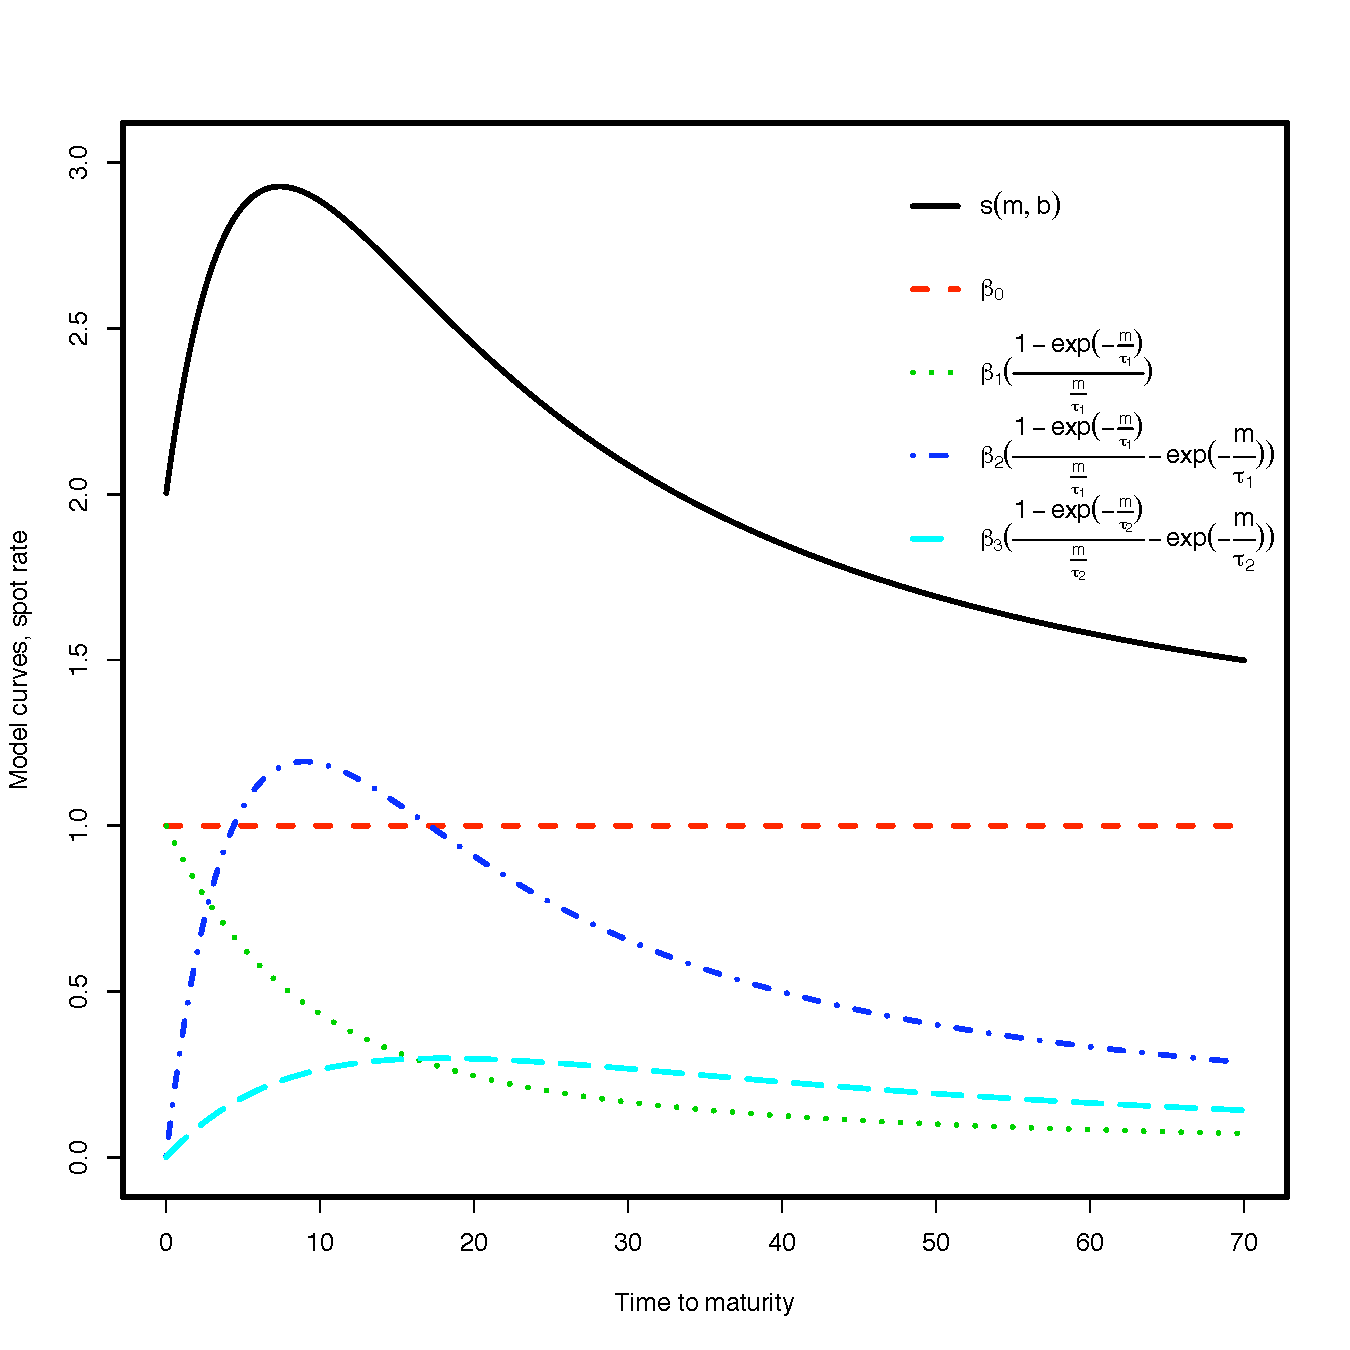
\includegraphics[width=0.7\textwidth]{curveshape}
\end{figure}

\begin{itemize}
\item $\beta_0>0$ is the asymptotic value of the spot rate function $\lim_{m_{ij}\to\infty}s(m_{ij},\bm{\beta})$, which can be seen as the long-term interest rate.
\item $\beta_1$ determines the rate of convergence with which the spot rate function approaches its long-term trend, and $\beta_0+\beta_1$ is the starting value of the curve at the short end. The slope will be negative if $\beta_1>0$ and vice versa.
\item $\beta_2$ determines the size and the form of the hump. $\beta_2 >0$  results in a hump at  $\tau_1$, whereas $\beta_2<0$ produces a $U$-shape.
\item $\tau_1>0$ specifies the location of the first hump or the U-shape on the curve.
\item $\beta_3$, analogously to $\beta_2$, determines the size and form of the second hump.
\item $\tau_2>0$ specifies the position of the second hump.
\end{itemize}

The discount factor for any maturity $m_{ij}$ can be calculated as follows:

\begin{displaymath}
\delta(m_{ij}, \bm{\beta})=e^{-m_{ij}s(m_{ij},\bm{\beta})}\,,
\end{displaymath}

where $s(m_{ij},\bm{\beta})$ is the Nelson/Siegel or Svensson spot rate function defined in \eqref{eq:nelson-spot} and \eqref{eq:svensson-spot}. We optimize the objective function in \eqref{eq:optimalparam}. The above specification of the discount function leads to a nonlinear optimization problem. Good starting values for the parameter vector are important to find a global minimum. Instead of minimizing pricing errors, it is common to minimize the yield errors. The yield-to-maturities of the theoretical bond prices can easily be calculated numerically, because \eqref{eq:yield} has only one real root. 

When minimizing the unweighted price errors, bonds with a longer maturity get a higher weighting, because they are more sensitive to changes in prices, which leads to a less accurate fit at the short end. Solutions to this heteroskedasticity problem are to use weights for the price errors, or to minimize the yield errors. A possible specification for the weights is based on the inverse of the duration as in \eqref{eq:durationweight} \citep[see][]{Bliss1997}.


%%% Local Variables: 
%%% mode: latex
%%% TeX-master: "jss-termstrc"
%%% End: 

\section{Cubic splines}
\label{sec:cubic-splines}

\begin{itemize}
\item \cite{McCulloch1971, McCulloch1975}
\item \cite{}
\end{itemize}


	$$\bm{G}_{\left[n \times m\right]} = \{  g_{ij}(m_{ij},l) \} \qquad   l = 1\dots s ; s= INT[\sqrt{m}]$$

	

	$$\bm{X}_{\left[m \times s\right]}=\{ \bm{x}_{\left[m \times 1\right]} \} \qquad  \bm{x}_{\left[m \times 1\right]} = \left( \iota_{\left[1\times n\right]} \bm{C}_{\left[n\times m\right]} \cdot \bm{G}_{\left[n\times m\right]}(l) \right)^t$$

	

	$$\bm{y}_{\left[m \times 1\right]}=  \bm{p}^d_{\left[1\times m\right]}  - \iota_{\left[1\times n\right]} \bm{C}_{\left[n\times m\right]}   $$

	

	$$\bm{\hat \alpha}_{\left[s \times 1\right]}= \left( \bm{X}^t   \bm{X}\right )^{-1}\bm{X}^t \bm{y}$$



%%% Local Variables: 
%%% mode: latex
%%% TeX-master: "jss-termstrc"
%%% End: 

\subsection{Parametric methods}

We load the package with the following command.


\begin{Schunk}
\begin{Sinput}
R> library("termstrc")
\end{Sinput}
\end{Schunk}

In the next steps we load the data set \proglang{govbonds} and explore its structure.

\begin{Schunk}
\begin{Sinput}
R> data(govbonds)
R> summary(govbonds)
\end{Sinput}
\begin{Soutput}
        Length Class  Mode
GERMANY 8      -none- list
AUSTRIA 8      -none- list
BELGIUM 8      -none- list
FINLAND 8      -none- list
FRANCE  8      -none- list
SPAIN   8      -none- list
\end{Soutput}
\end{Schunk}

It includes data for government bonds of six European countries. The bonds are classified by their \emph{International Securities Identifying Number (ISIN)}, and all the necessary information on the future cash flows is given.

\begin{Schunk}
\begin{Sinput}
R> str(govbonds$GERMANY)
\end{Sinput}
\begin{Soutput}
List of 8
 $ ISIN        : chr [1:52] "DE0001141414" "DE0001137131" "DE0001141422" "DE0001137149" ...
 $ MATURITYDATE:Class 'Date'  num [1:52] 13924 13952 13980 14043 14064 ...
 $ ISSUEDATE   :Class 'Date'  num [1:52] 11913 13215 12153 13298 10411 ...
 $ COUPONRATE  : num [1:52] 0.0425 0.0300 0.0300 0.0325 0.0413 ...
 $ PRICE       : num [1:52] 100.0  99.9  99.8  99.8 100.1 ...
 $ ACCRUED     : num [1:52] 4.09 2.66 2.43 2.07 2.39 ...
 $ CASHFLOWS   :List of 3
  ..$ ISIN: chr [1:384] "DE0001141414" "DE0001137131" "DE0001141422" "DE0001137149" ...
  ..$ CF  : num [1:384] 104 103 103 103 104 ...
  ..$ DATE:Class 'Date'  num [1:384] 13924 13952 13980 14043 14064 ...
 $ TODAY       :Class 'Date'  num 13908
\end{Soutput}
\end{Schunk}

Suppose, we want to perform a zero-coupon yield curve estimation for several countries with the \cite{Nelson1987} method minimizing the duration weighted pricing errors. The sample of bonds is restricted to a maximum maturity of 30 years. 

\begin{Schunk}
\begin{Sinput}
R> group <- c("GERMANY", "FRANCE", "BELGIUM", "SPAIN")
R> bonddata <- govbonds
R> matrange <- c(0, 30)
R> method <- "Nelson/Siegel"
R> fit <- "prices"
R> weights <- "duration"
R> b <- matrix(rep(c(0, 0, 0, 1), 4), nrow = 4, byrow = TRUE)
R> rownames(b) <- group
R> colnames(b) <- c("beta0", "beta1", "beta2", "tau1")
R> x <- nelson_estim(group, bonddata, matrange, method, fit, weights, 
...    b)
\end{Sinput}
\end{Schunk}

Now, let us have a look at the results.

\begin{Schunk}
\begin{Sinput}
R> x
\end{Sinput}
\begin{Soutput}
---------------------------------------------------
Parameters for Nelson/Siegel, Svensson estimation:

Method: Nelson/Siegel 
Fitted: prices 
Weights: duration 

---------------------------------------------------

           GERMANY      FRANCE      BELGIUM        SPAIN
beta_0  0.05130485  0.05118613  0.052087336  0.052729208
beta_1 -0.01268934 -0.01242461 -0.008902787  0.002793828
beta_2 -0.03215030 -0.03036739 -0.036863081 -0.047882039
tau_1   2.68940959  2.54290443  2.185687965  1.863315577
\end{Soutput}
\end{Schunk}

The summary method gives goodness of fit measures for the pricing and the yield errors. Moreover, it shows the convergence information from the solver to check whether a solution to the nonlinear optimization problem has been found.

\begin{Schunk}
\begin{Sinput}
R> summary(x)
\end{Sinput}
\begin{Soutput}
---------------------------------------------------
Goodness of fit:
---------------------------------------------------

                  GERMANY       FRANCE     BELGIUM       SPAIN
RMSE-Prices  0.3578726990 0.2214576932 2.222911540 2.011818325
AABSE-Prices 0.2030132843 0.1184783548 0.776049451 1.724348860
RMSE-Yields  0.0008413222 0.0003923194 0.005007131 0.008045454
AABSE-Yields 0.0005305512 0.0002735921 0.002114202 0.005710166


---------------------------------------------------
Convergence information:
---------------------------------------------------

        Convergence ()
GERMANY "converged"   
FRANCE  "converged"   
BELGIUM "converged"   
SPAIN   "converged"   

        Solver message            
GERMANY "relative convergence (4)"
FRANCE  "relative convergence (4)"
BELGIUM "relative convergence (4)"
SPAIN   "relative convergence (4)"
\end{Soutput}
\end{Schunk}


%<<echo=FALSE>>=
%pdf("fig_eurospotcurves.pdf", width=8, height=6)
%plot(x,multiple=TRUE,errors="none")
%dev.off()
%@

Our package offers several options to plot the results, e.g. spot rate, forward rate, discount and spread curves. Figure \ref{fig:spotcurves} shows the estimated zero-coupon yield curves. The dashed lines indicate that the curve was extrapolated, which is possible with the \cite{Nelson1987} and \cite{Svensson1994} approach.

\begin{figure}[htb]
\centering
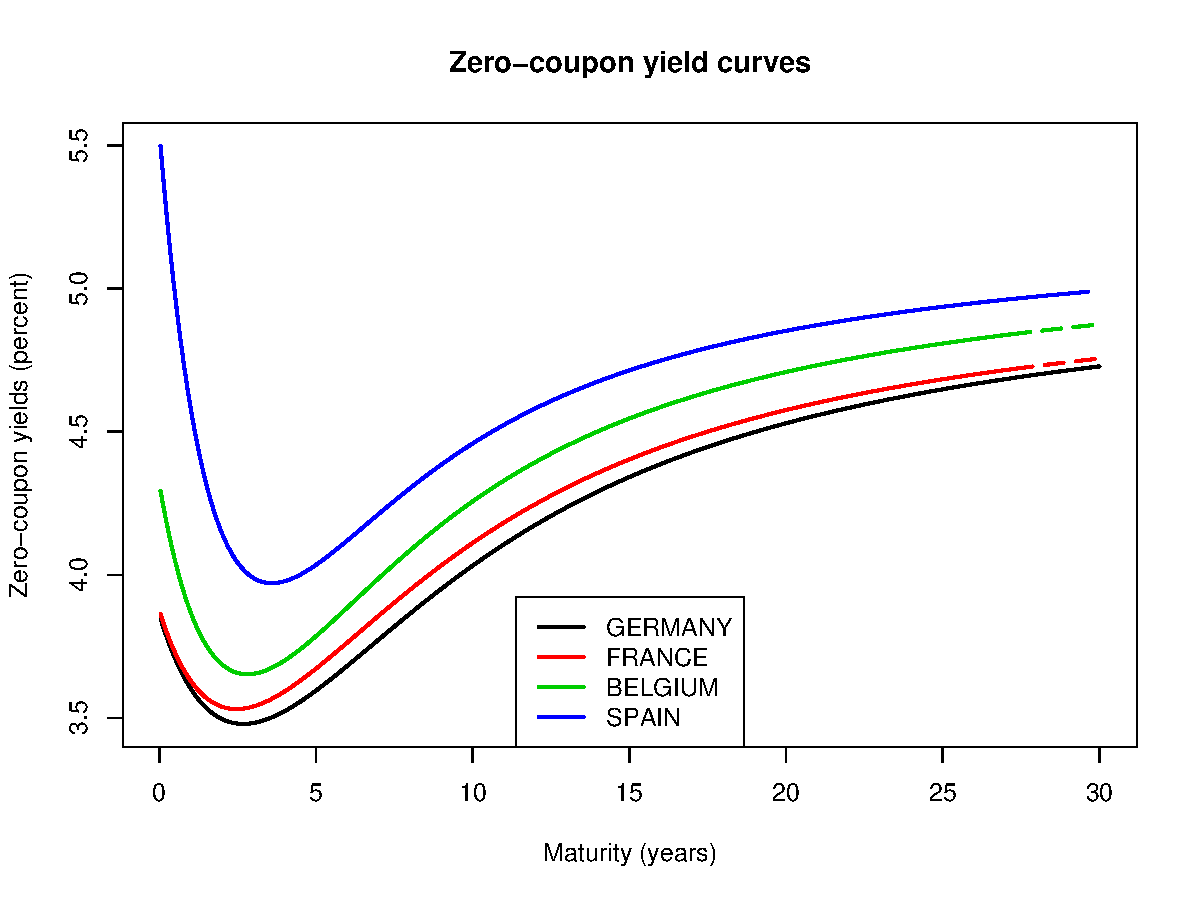
\includegraphics[width=0.7\textwidth]{fig_eurospotcurves}
\caption{Zero-coupon yield curves estimated with Nelson/Siegel}
\label{fig:spotcurves}
\end{figure}


\subsection{Spline-based methods}

In this section, we to demonstrate how to estimate the term structure of interest rates with the \cite{McCulloch1975} cubic splines approach applied to French governement bonds.

\begin{Schunk}
\begin{Sinput}
R> y <- splines_estim(c("FRANCE"), govbonds, c(0, 30))
R> y
\end{Sinput}
\begin{Soutput}
---------------------------------------------------
Parameters for Cubic splines estimation:

[1] "FRANCE:"
      alpha 1       alpha 2       alpha 3       alpha 4       alpha 5 
 0.0136620572 -0.0018022601 -0.0003772906  0.0001867318  0.0010633259 
      alpha 6       alpha 7 
 0.0014693772 -0.0408879155 
\end{Soutput}
\end{Schunk}

The summary method shows details from the OLS estimation of the parameters and the goodness of fit measures.

\begin{Schunk}
\begin{Sinput}
R> summary(y)
\end{Sinput}
\begin{Soutput}
---------------------------------------------------
Goodness of fit:
---------------------------------------------------

                   FRANCE
RMSE-Prices  0.1819767236
AABSE-Prices 0.0820766103
RMSE-Yields  0.0005212926
AABSE-Yields 0.0002514331

---------------------------------------------------
Summary statistics for the fitted models:
---------------------------------------------------

$FRANCE

Call:
lm(formula = -Y[[k]] ~ X[[k]] - 1)

Residuals:
      Min        1Q    Median        3Q       Max 
-0.663324 -0.030923 -0.007992  0.041845  0.908719 

Coefficients:
          Estimate Std. Error t value Pr(>|t|)    
alpha 1  0.0136621  0.0072072   1.896    0.066 .  
alpha 2 -0.0018023  0.0020768  -0.868    0.391    
alpha 3 -0.0003773  0.0008139  -0.464    0.646    
alpha 4  0.0001867  0.0002862   0.652    0.518    
alpha 5  0.0010633  0.0001208   8.804 1.66e-10 ***
alpha 6  0.0014694  0.0002102   6.989 3.39e-08 ***
alpha 7 -0.0408879  0.0032007 -12.774 6.14e-15 ***
---
Signif. codes:  0 '***' 0.001 '**' 0.01 '*' 0.05 '.' 0.1 ' ' 1 

Residual standard error: 0.1989 on 36 degrees of freedom
Multiple R-squared:     1,	Adjusted R-squared:     1 
F-statistic: 3.211e+05 on 7 and 36 DF,  p-value: < 2.2e-16 
\end{Soutput}
\end{Schunk}

% <<echo=FALSE>>=
% pdf("fig_frenchspotcurve.pdf", width=8, height=6)
% plot(y,errors="none")
% dev.off()
% @

Figure \ref{fig:frenchspotcurve} shows the yield-to-maturities and the estimated zero-coupon yield curve together with the automatically selected knot points.

\begin{figure}[htb]
\centering
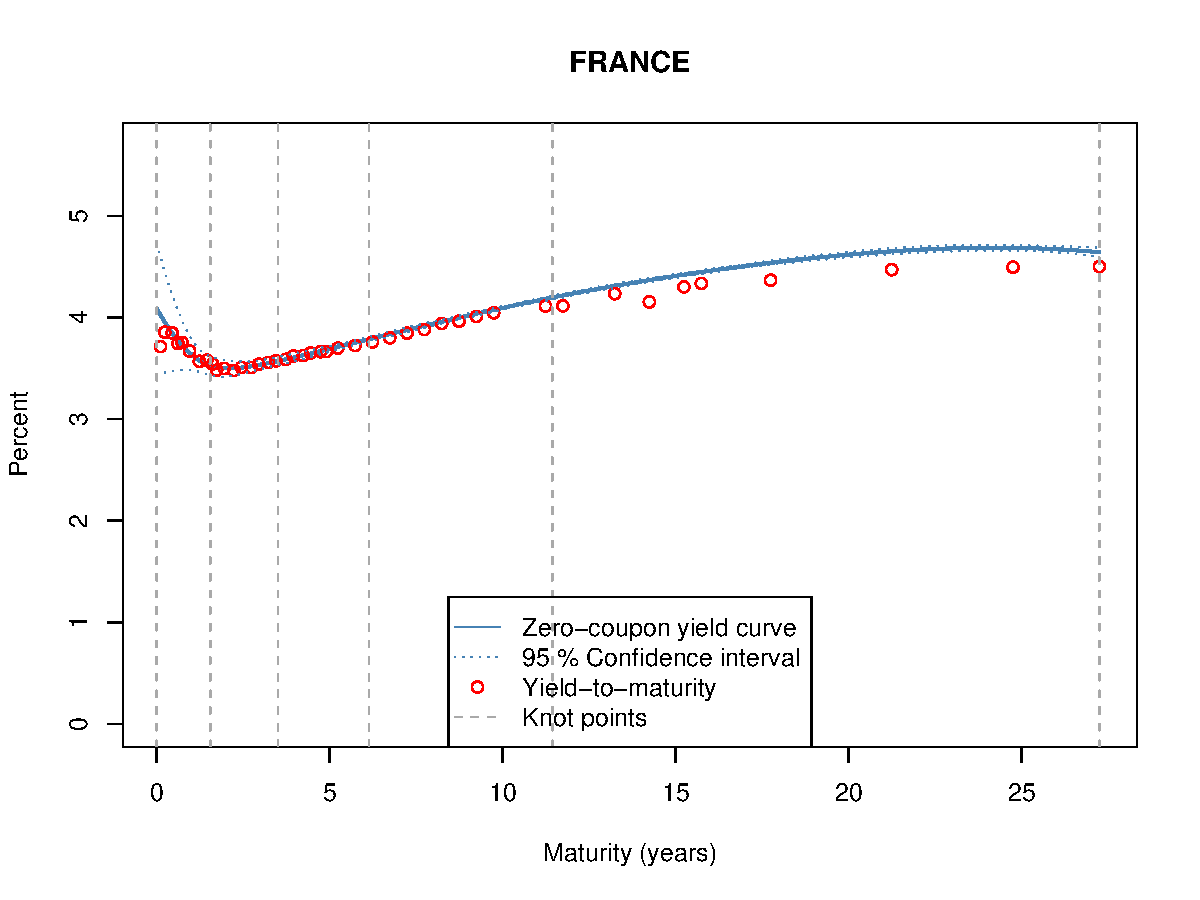
\includegraphics[width=0.8\textwidth]{fig_frenchspotcurve}
\caption{Zero-coupon yield curve for French government bonds estimated with cubic splines}
\label{fig:frenchspotcurve}
\end{figure}

% \begin{figure}[htb]
% \caption{Pricing errors for French government bonds}  
% \begin{center}
% <<fig=TRUE, echo=FALSE>>=
% plot(y,ctype="none", inset=c(0.2, 0.4))
% @
% \end{center}
% \end{figure}

%<<echo=FALSE, fig=FALSE>>=
%pdf("fig_pricingerrors.pdf", width=12, height=8)
%plot(y,ctype="none", inset=c(0.2, 0.4))
%dev.off()
%@

As we can see in Figure \ref{fig:pricingerrors}, there seems to be a misspricing of two bonds. They can be removed and the estimation is redone.

\begin{figure}[htb]
\centering  
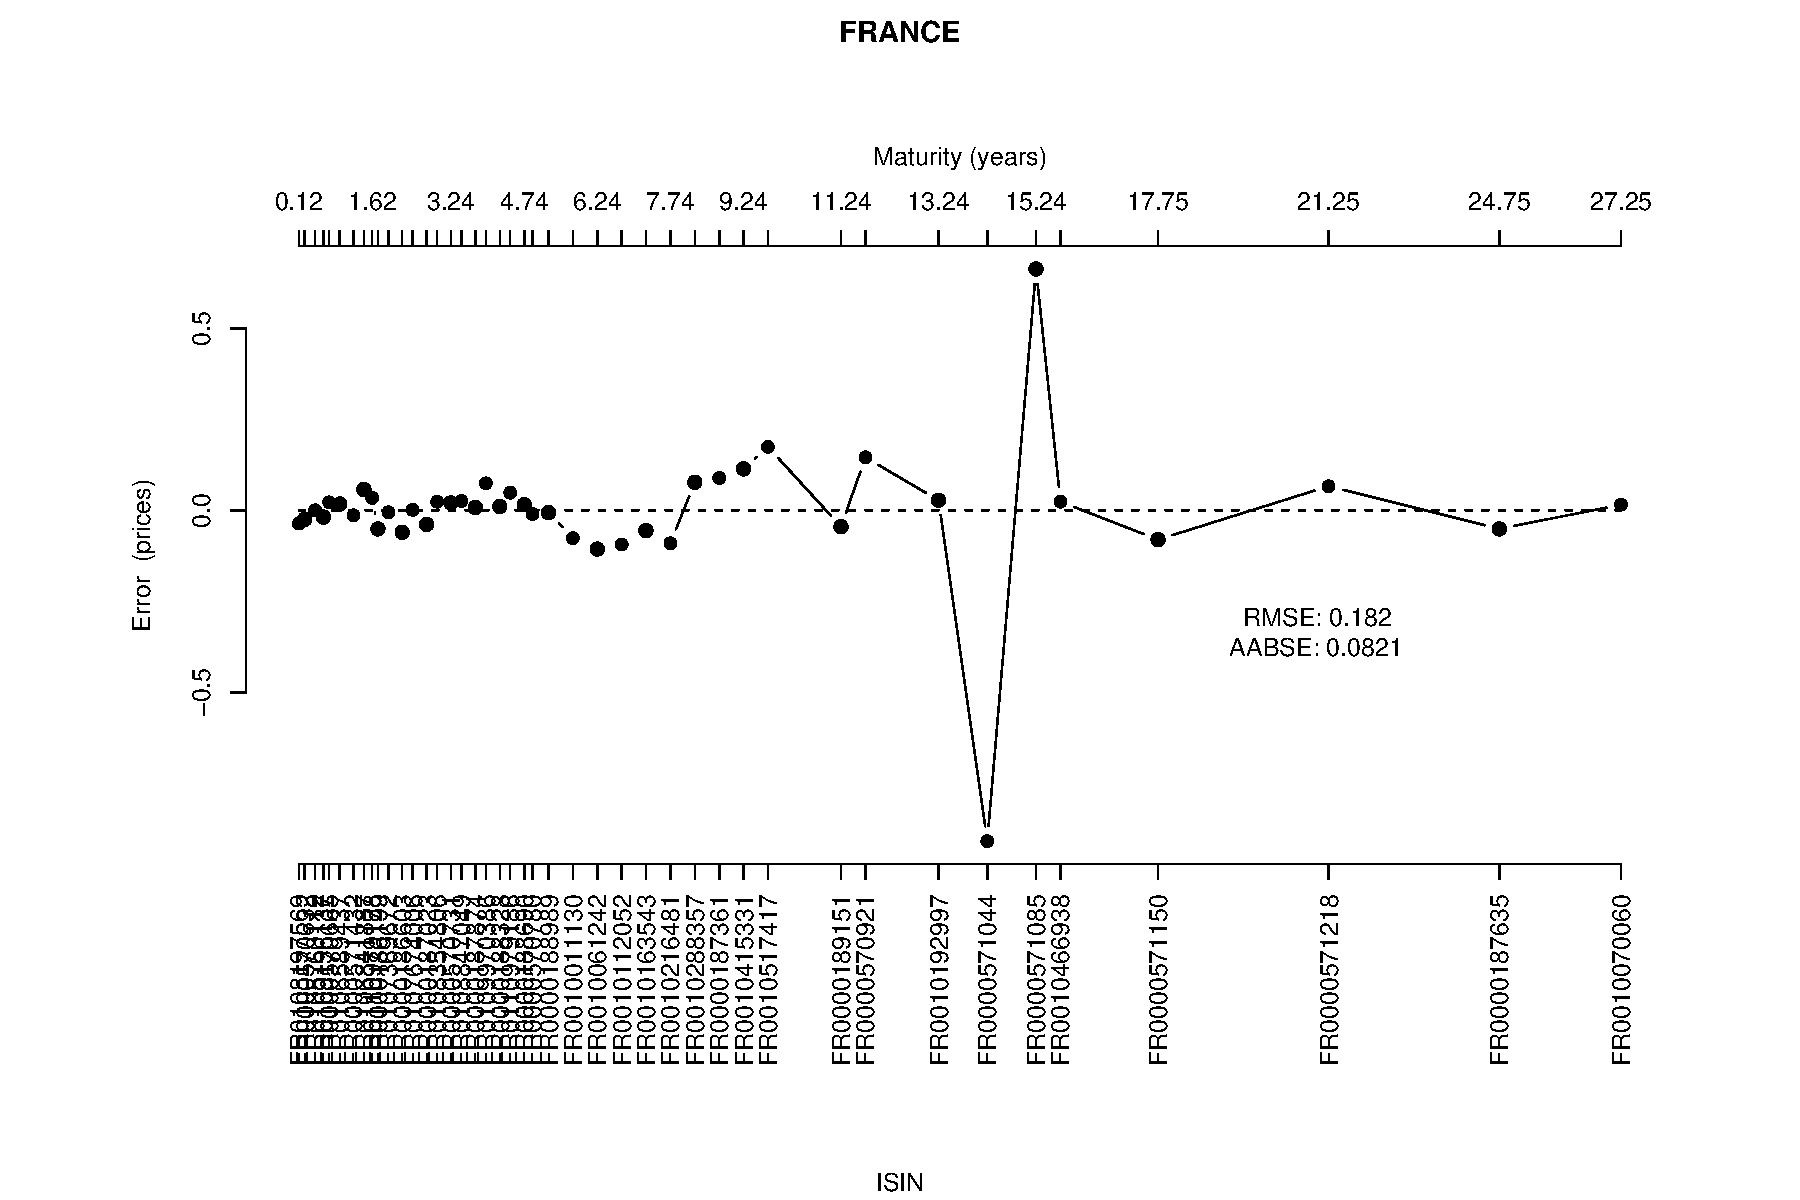
\includegraphics[width=0.8\textwidth]{fig_pricingerrors}
\caption{Pricing errors for French government bonds} 
\label{fig:pricingerrors}
\end{figure}

As expected, the goodness of fit is improved.

\begin{Schunk}
\begin{Sinput}
R> z <- splines_estim(c("FRANCE"), rm_bond(bonddata, c("FR0000571044", 
...    "FR0000571085"), "FRANCE"), c(0, 30))
\end{Sinput}
\end{Schunk}
\begin{Schunk}
\begin{Sinput}
R> summary(z)
\end{Sinput}
\begin{Soutput}
---------------------------------------------------
Goodness of fit:
---------------------------------------------------

                   FRANCE
RMSE-Prices  0.0615589340
AABSE-Prices 0.0515614078
RMSE-Yields  0.0003452360
AABSE-Yields 0.0002025576

---------------------------------------------------
Summary statistics for the fitted models:
---------------------------------------------------

$FRANCE

Call:
lm(formula = -Y[[k]] ~ X[[k]] - 1)

Residuals:
     Min       1Q   Median       3Q      Max 
-0.10516 -0.03516 -0.01789  0.05302  0.14043 

Coefficients:
          Estimate Std. Error t value Pr(>|t|)    
alpha 1  8.886e-03  1.558e-03   5.704 1.89e-06 ***
alpha 2 -9.269e-04  3.869e-04  -2.396   0.0221 *  
alpha 3 -5.500e-04  1.175e-04  -4.682 4.17e-05 ***
alpha 4  9.038e-04  3.307e-05  27.334  < 2e-16 ***
alpha 5  1.526e-03  5.085e-05  30.005  < 2e-16 ***
alpha 6 -3.921e-02  8.287e-04 -47.318  < 2e-16 ***
---
Signif. codes:  0 '***' 0.001 '**' 0.01 '*' 0.05 '.' 0.1 ' ' 1 

Residual standard error: 0.06663 on 35 degrees of freedom
Multiple R-squared:     1,	Adjusted R-squared:     1 
F-statistic: 2.856e+06 on 6 and 35 DF,  p-value: < 2.2e-16 
\end{Soutput}
\end{Schunk}






\clearpage
\section{Discussion}


\includegraphics[width=0.3in]{baustelle} discuss extensions of both methods

We 

\begin{itemize}
\item extensions for credit spread estimation \cite{Jankowitsch2004, Geyer2004}
\item extensions for splines: exponential splines by \cite{Vasicek1982} (leads to more realisitc shapes of the forward curve), \cite{Adams1994} obtain maximum smoothness, \cite{Fisher1995, Waggoner1997, Anderson1999 }
\end{itemize}


\begin{itemize}
\item parametric cubic splines \cite{McCulloch1971, McCulloch1975}
\item non-parametric splines \cite{Adams1994,Fisher1995, Waggoner1997, Tanggaard1997, Shea1985}
\item \cite{Shea1985} mentions unstable fluctuating forward rates in \cite{McCulloch1975} cubic splines

\end{itemize}


\includegraphics[width=0.3in]{baustelle} describe available other software solutions

%%% Local Variables: 
%%% mode: latex
%%% TeX-master: "jss-termstrc"
%%% End: 

\section{Conclusion}
\label{sec:conclusion}

In this paper, we presented the \proglang{R} extension package \pkg{termstrc}. It provides functions for the estimation of zero-coupon yield curves from market data of coupon bonds. The package covers the two most widely-used approaches in practice and provides a simple interface to them. The results contain detailed summaries about the estimation, as well as graphical outputs of spot, forward, discount and spread curves.


\section*{Acknowledgments}

The authors want to thank Alois Geyer and Kurt Hornik for their comments on the package and the paper.



%%% Local Variables: 
%%% mode: latex
%%% TeX-master: "jss-termstrc"
%%% End: 


We use \cite{R2007}.

%\nocite{*}
%\listoftables
%\listoffigures
\bibliographystyle{jss}
\bibliography{termstrc}

\end{document}



%%% Local Variables: 
%%% mode: latex
%%% TeX-master: "jss-termstrc"
%%% End: 
